\subsection{Geometry and material properties}
\label{sub:geometry_and_material_properties}

\begin{center}
    \huge{Explain the safety factor influence on the choice of coordinates [X, Y]}
\end{center}

At first the FEM model was imported in adequate \texttt{MATLAB} data structures, containing in particular the geometrical and material properties of the system.

The output of this first step is a schematized version of the harbour crane, as shown in Figure \ref{fig:harbour-crane-scheme}.

\begin{figure}[H]
    \centering
    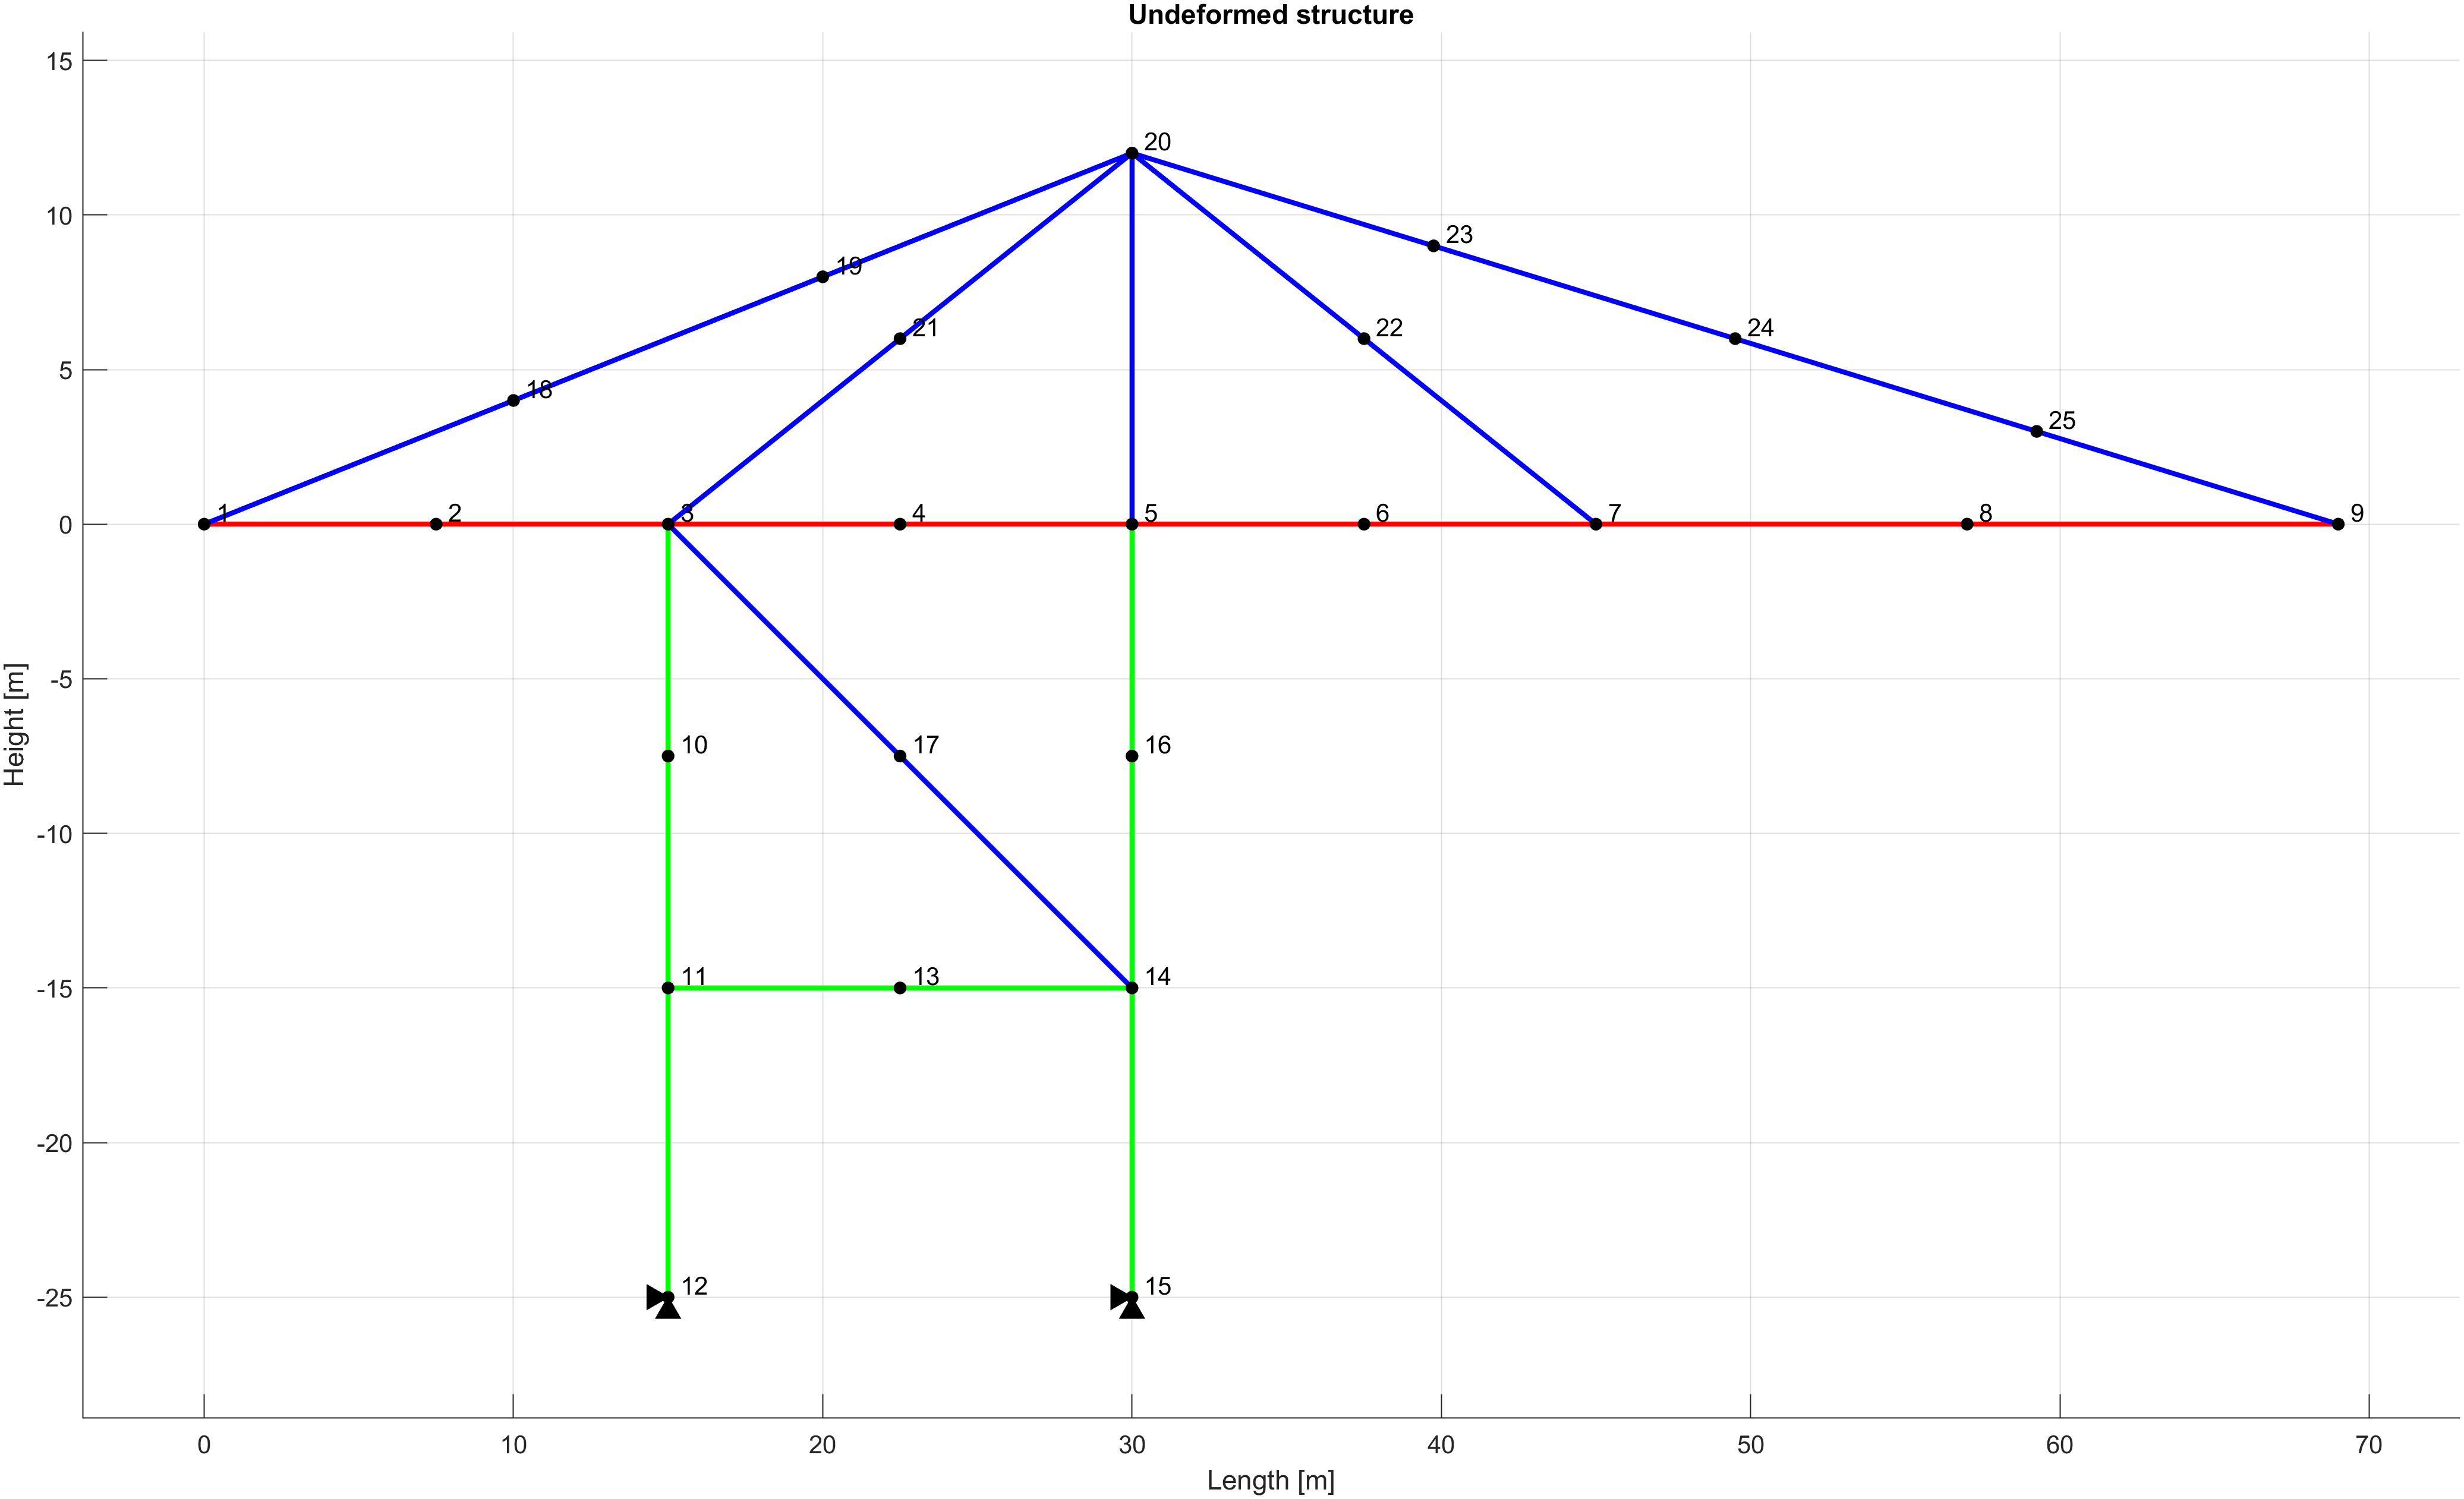
\includegraphics[width=0.7\textwidth]{img/MATLAB/undeformed-structure.png}
    \caption{Harbour crane scheme}
    \label{fig:harbour-crane-scheme}
\end{figure}

As suggested/requested by the assignment, the harbour crane was modelled as a 2D frame structure composed of beam elements.
As an assumption, the joints nodes number \textbf{\#1} and \textbf{\#9} were assumed to be rigid connections, while in reality those elements are usually not capable of transmit bending moments, but only axial forces.
This assumption was made to simplify the model and the analysis.
However, the model could be easily modified to include the possibility of free relative rotations in those joints by adding another degree of freedom to the system.

With respect to the schematic representation of the crane of Figure \ref{fig:harbour-crane-scheme}, the parameters of the structure are provided in Table \ref{tab:parameters}.

\begin{table}[H]
    \centering
    \begin{tabular}{|r|c|c|c|}
        \hline
        ~           & \textbf{m [kg/m]} & \textbf{EA [N]} & \textbf{EJ [Nm$^2$]} \\
        \hline
        Red beams   & $312$             & $8.2E9$         & $1.4E9$              \\
        Green beams & $200$             & $5.4E9$         & $4.5E8$              \\
        Blue beams  & $90$              & $2.4E9$         & $2.0E8$              \\
        \hline
    \end{tabular}
    \caption{Parameters of the structure}
    \label{tab:parameters}
\end{table}

For the rest of the analysis, we will assume a proportional damping matrix $[C] = \alpha [M] + \beta [K]$ with $\alpha = 0.01 [s/(m \times kg)]$ and $\beta = 2E-4 [s^3 / (m \times kg)]$